\begin{frame}
\frametitle{Implementações}
\centering
\textbf{Implementações e Outras Contribuições}
\end{frame}

\section{Implementações}
\subsection{Moore}
\begin{frame}
\frametitle{Implementações}
\framesubtitle{Grafos de Moore}
Um Grafo de {\it Moore} é um Grafo regular de grau $d$ e distância $k$ tal que o número de vértices é igual ao limitante superior: $$1 + d\sum_{i=0}{k-1}(d-1)^i$$
\end{frame}


\begin{frame}
\frametitle{Implementações}
\framesubtitle{Grafos de Moore}
\begin{itemize}
    \item{Diâmetro 2, só são possíveis para os valores de $k$ igual a 2, 3, 7 ou 57 [Hoffman e Singleton, 1960]}
    \item{Não existem grafos de Moore com $\Delta \geq 3$ e $d\geq 3$, ou seja eles possuem diâmetro no máximo 2 [Bannai, 1973]}
\end{itemize}
\end{frame}

\begin{frame}
\frametitle{Implementações}
\framesubtitle{Grafo de Moore - $k={2,3,7}$}
Grafos de Moore conhecidos:
\begin{itemize}
    \item{$k=2$ Ciclo de tamanho 5}
    \item{$k=3$ Petersen}
    \item{$k=7$ Hoffman-Singleton}
\end{itemize}
\end{frame}

\begin{frame}
\frametitle{Implementações}
\framesubtitle{Grafo de Moore 57-regular - Sabemos}
\begin{itemize}
    \item{Sua existência permanece em aberto desde 1960}
    \item{57 regular, 3250 vértices, 92625 arestas, diâmetro 2 e cintura 5}
    \item{Não é distância-transitivo [Aschbacher, 1971]}
    \item{Não é vértice-transitivo [Cameron, 1983]}
    \item{Possui ao menos 375 automorfismo [Macaj, 2010]}
\end{itemize}
\end{frame}



\begin{frame}
\frametitle{Implementações}
\framesubtitle{Algoritmo - Grafos de Moore - Construção esqueleto}
\begin{figure}[h]
\centering
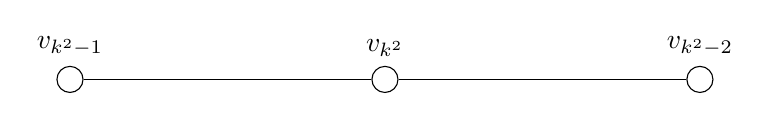
\begin{tikzpicture}[scale=0.8]
\node[circle,draw,label=above:$v_{k^2-2}$] (v2) at (5,0) {};
\node[circle,draw,label=above:$v_{k^2}$] (v1) at (0,0) {};
\node[circle,draw,label=above:$v_{k^2-1}$] (v3) at (-5,0) {};
\draw  (v1) edge (v2);
\draw  (v1) edge (v3);
\end{tikzpicture}
\label{fig-execucao-moore}
\end{figure}
\end{frame}

\begin{frame}
\frametitle{Implementações}
\framesubtitle{Algoritmo - Grafos de Moore - Construção esqueleto}
%\begin{turn}{-90}
\begin{figure}[h]
\centering
\begin{tikzpicture}[scale=0.8]
\node[circle,draw,label=above:$v_{k^2-2}$,fill] (v2) at (5,0) {};
\node[circle,draw,label=below:$v_{0}$] (v4) at (4,-3.5) {};
\node[circle,draw,label=above:$v_{k^2}$] (v1) at (0,0) {};
\node[circle,draw,label=above:$v_{k^2-1}$,fill] (v3) at (-5,0) {};
\node[circle,draw,label=below:$v_{k-1}$] (v7) at (-4,-3.5) {};
\node[circle,draw,label=below:$v_{1}$] (v5) at (5,-5) {};
\node[circle,draw,label=below:$v_{k-2}$] (v6) at (6,-6.5) {};
\node[circle,draw,label=below:$v_{k}$] (v8) at (-5,-5) {};
\node[circle,draw,label=below:$v_{2k-3}$] (v9) at (-6,-6.5) {};
\draw  (v1) edge (v2);
\draw  (v1) edge (v3);
\draw  (v2) edge (v4);
\draw  (v2) edge (v5);
\draw  (v2) edge (v6);
\draw  (v3) edge (v7);
\draw  (v3) edge (v8);
\draw  (v3) edge (v9);
\draw[dotted]  (v5) edge (v6);
\draw[dotted]  (v8) edge (v9);
\end{tikzpicture}
\label{fig-execucao-moore}
\end{figure}
%\end{turn}
\end{frame}

\begin{frame}
\frametitle{Implementações}
\framesubtitle{Algoritmo - Grafos de Moore - Construção esqueleto}
%\begin{turn}{-90}
\begin{figure}[h]
\centering
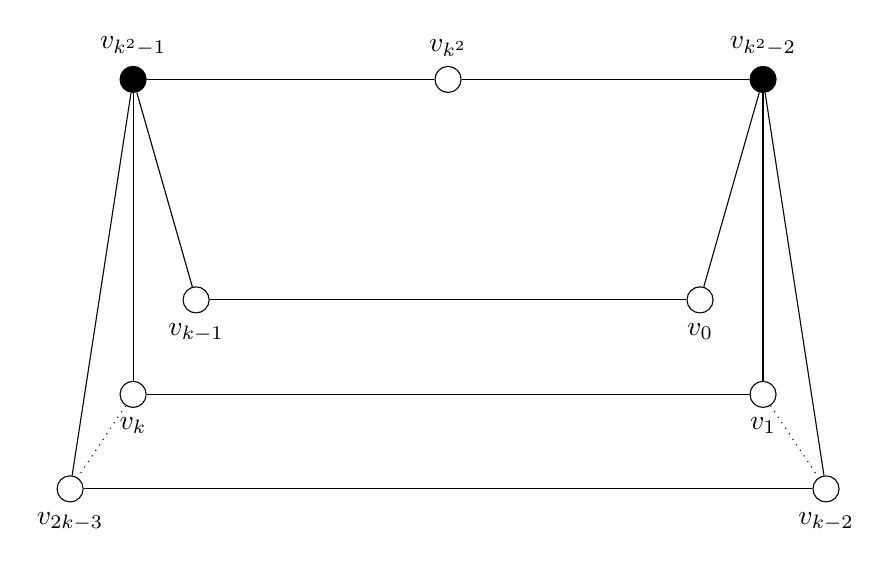
\begin{tikzpicture}[scale=0.8]
\node[circle,draw,label=above:$v_{k^2-2}$,fill] (v2) at (5,0) {};
\node[circle,draw,label=below:$v_{0}$] (v4) at (4,-3.5) {};
\node[circle,draw,label=above:$v_{k^2}$] (v1) at (0,0) {};
\node[circle,draw,label=above:$v_{k^2-1}$,fill] (v3) at (-5,0) {};
\node[circle,draw,label=below:$v_{k-1}$] (v7) at (-4,-3.5) {};
\node[circle,draw,label=below:$v_{1}$] (v5) at (5,-5) {};
\node[circle,draw,label=below:$v_{k-2}$] (v6) at (6,-6.5) {};
\node[circle,draw,label=below:$v_{k}$] (v8) at (-5,-5) {};
\node[circle,draw,label=below:$v_{2k-3}$] (v9) at (-6,-6.5) {};
\draw  (v1) edge (v2);
\draw  (v1) edge (v3);
\draw  (v2) edge (v4);
\draw  (v2) edge (v5);
\draw  (v2) edge (v6);
\draw  (v3) edge (v7);
\draw  (v3) edge (v8);
\draw  (v3) edge (v9);
\draw  (v4) edge (v7);
\draw  (v5) edge (v8);
\draw  (v6) edge (v9);
\draw[dotted]  (v5) edge (v6);
\draw[dotted]  (v8) edge (v9);
\end{tikzpicture}
\label{fig-execucao-moore}
\end{figure}
%\end{turn}
\end{frame}



\begin{frame}
\frametitle{Implementações}
\framesubtitle{Algoritmo - Grafos de Moore - Construção esqueleto}
%\begin{turn}{-90}
\begin{figure}[h]
\centering
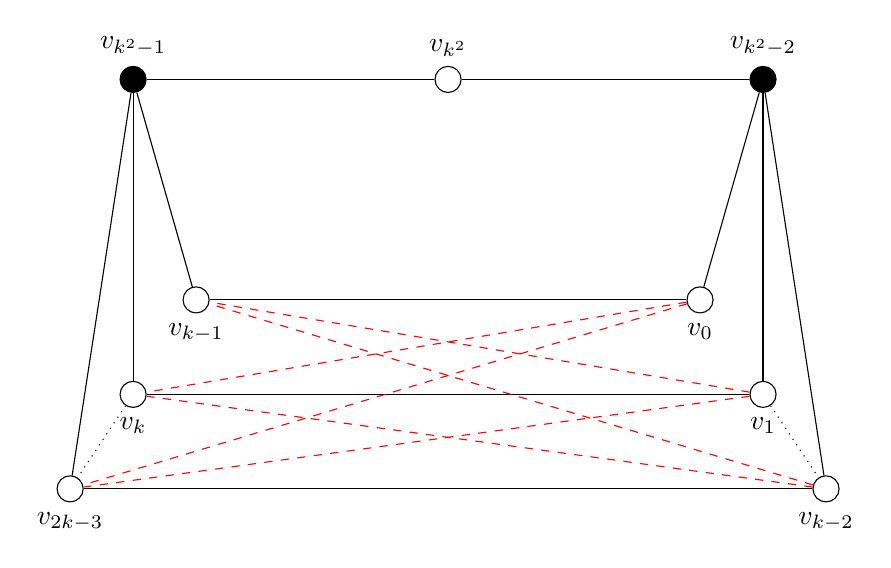
\begin{tikzpicture}[scale=0.8]
\node[circle,draw,label=above:$v_{k^2-2}$,fill] (v2) at (5,0) {};
\node[circle,draw,label=below:$v_{0}$] (v4) at (4,-3.5) {};
\node[circle,draw,label=above:$v_{k^2}$] (v1) at (0,0) {};
\node[circle,draw,label=above:$v_{k^2-1}$,fill] (v3) at (-5,0) {};
\node[circle,draw,label=below:$v_{k-1}$] (v7) at (-4,-3.5) {};
\node[circle,draw,label=below:$v_{1}$] (v5) at (5,-5) {};
\node[circle,draw,label=below:$v_{k-2}$] (v6) at (6,-6.5) {};
\node[circle,draw,label=below:$v_{k}$] (v8) at (-5,-5) {};
\node[circle,draw,label=below:$v_{2k-3}$] (v9) at (-6,-6.5) {};
\draw  (v1) edge (v2);
\draw  (v1) edge (v3);
\draw  (v2) edge (v4);
\draw  (v2) edge (v5);
\draw  (v2) edge (v6);
\draw  (v3) edge (v7);
\draw  (v3) edge (v8);
\draw  (v3) edge (v9);
\draw  (v4) edge (v7);
\draw  (v5) edge (v8);
\draw  (v6) edge (v9);
\draw[dashed] (v4) edge[red] (v8);
\draw[dashed]  (v5) edge[red] (v7);
\draw[dashed]  (v6) edge[red] (v7);
\draw[dashed]  (v4) edge[red] (v9);
\draw[dashed]  (v5) edge[red] (v9);
\draw[dashed]  (v6) edge[red] (v8);
\draw[dotted]  (v5) edge (v6);
\draw[dotted]  (v8) edge (v9);
\end{tikzpicture}
\label{fig-execucao-moore}
\end{figure}
%\end{turn}
\end{frame}


\begin{frame}
\frametitle{Implementações}
\framesubtitle{Algoritmo - Grafos de Moore - Construção esqueleto}
\centering
\begin{turn}{-90}
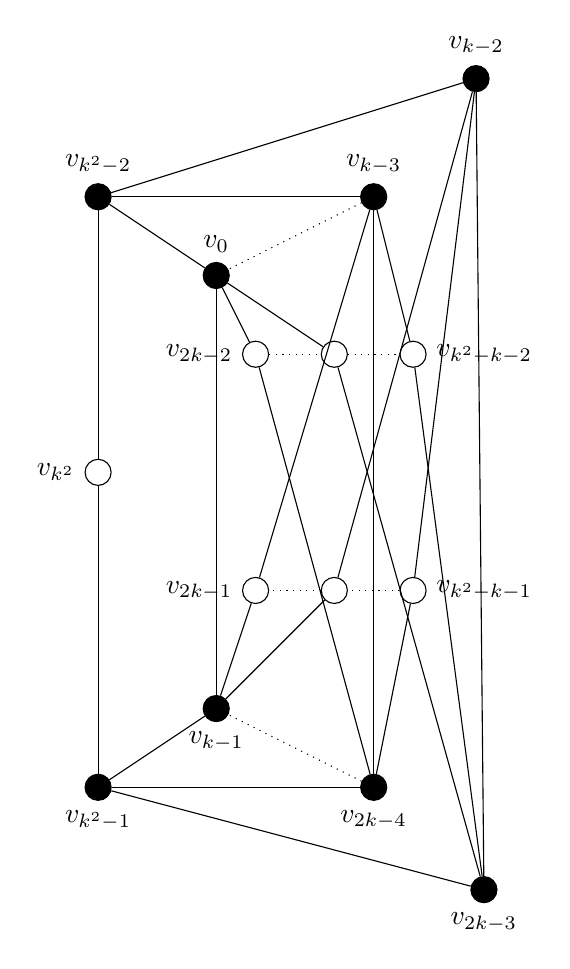
\begin{tikzpicture}
\node[circle,draw,label=$v_{k^2-2}$,fill] (v2) at (-2.5,4) {};
\node[circle,draw,label=$v_{0}$,fill] (v4) at (-1,3) {};
\node[circle,draw,label=left:$v_{k^2}$] (v1) at (-2.5,0.5) {};
\node[circle,draw,label=below:$v_{k^2-1}$,fill] (v3) at (-2.5,-3.5) {};
\node[circle,draw,label=below:$v_{k-1}$,fill] (v7) at (-1,-2.5) {};
\node[circle,draw,label=$v_{k-3}$,fill] (v5) at (1,4) {};
\node[circle,draw,label=$v_{k-2}$,fill] (v6) at (2.3,5.5) {};
\node[circle,draw,label=below:$v_{2k-4}$,fill] (v8) at (1,-3.5) {};
\node[circle,draw,label=below:$v_{2k-3}$,fill] (v9) at (2.4,-4.8) {};
\draw  (v1) edge (v2);
\draw  (v1) edge (v3);
\draw  (v2) edge (v4);
\draw  (v2) edge (v5);
\draw  (v2) edge (v6);
\draw  (v3) edge (v7);
\draw  (v3) edge (v8);
\draw  (v3) edge (v9);
\draw  (v4) edge (v7);
\draw  (v5) edge (v8);
\draw  (v6) edge (v9);
\draw[dotted]  (v5) edge (v4);
\draw[dotted]  (v8) edge (v7);
\node[draw,circle,label=left:$v_{2k-2}$] (v10) at (-0.5,2) {};
\node[draw,circle,label=left:$v_{2k-1}$] (v11) at (-0.5,-1) {};
\node[draw,circle] (v12) at (0.5,2) {};
\node[draw,circle] (v13) at (0.5,-1) {};
\node[draw,circle,label=right:$v_{k^2-k-1}$] (v15) at (1.5,-1) {};
\node[draw,circle,label=right:$v_{k^2-k-2}$] (v14) at (1.5,2) {};
\draw  (v4) edge (v10);
\draw  (v10) edge (v8);
\draw  (v7) edge (v11);
\draw  (v11) edge (v5);
\draw  (v4) edge (v12);
\draw  (v9) edge (v12);
\draw  (v7) edge (v13);
\draw  (v13) edge (v6);
\draw  (v5) edge (v14);
\draw  (v14) edge (v9);
\draw  (v8) edge (v15);
\draw  (v15) edge (v6);

\draw[dotted]  (v10) edge (v12);
\draw[dotted]  (v13) edge (v11);
\draw[dotted]  (v12) edge (v14);
\draw[dotted]  (v15) edge (v13);
\end{tikzpicture}
\end{turn}
\end{frame}


\begin{frame}
\frametitle{Implementações}
\framesubtitle{Algoritmo - Grafos de Moore - Esqueleto}
\centering
\begin{turn}{-90}
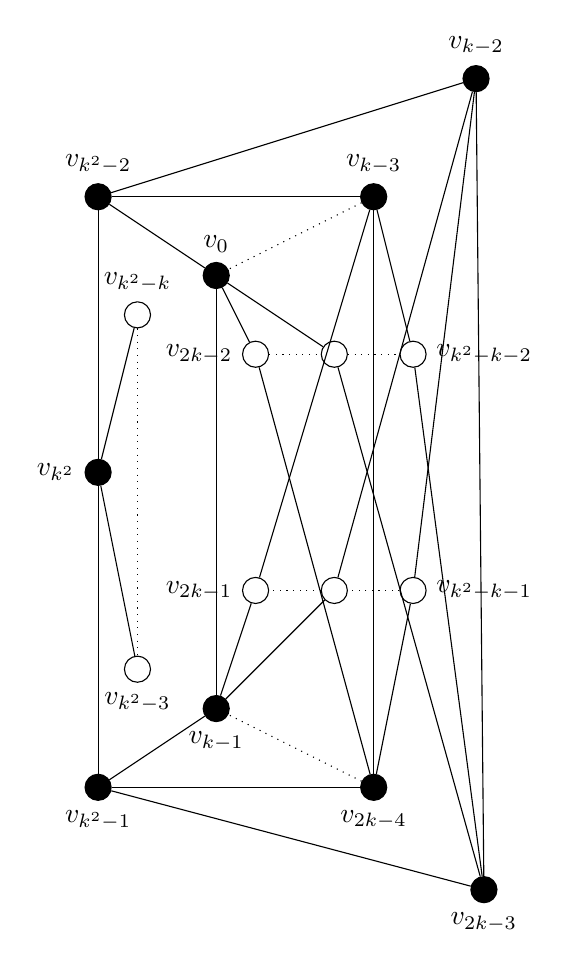
\begin{tikzpicture}
\node[circle,draw,label=$v_{k^2-2}$,fill] (v2) at (-2.5,4) {};
\node[circle,draw,label=$v_{0}$,fill] (v4) at (-1,3) {};
\node[circle,draw,label=left:$v_{k^2}$,fill] (v1) at (-2.5,0.5) {};
\node[circle,draw,label=below:$v_{k^2-1}$,fill] (v3) at (-2.5,-3.5) {};
\node[circle,draw,label=below:$v_{k-1}$,fill] (v7) at (-1,-2.5) {};
\node[circle,draw,label=$v_{k-3}$,fill] (v5) at (1,4) {};
\node[circle,draw,label=$v_{k-2}$,fill] (v6) at (2.3,5.5) {};
\node[circle,draw,label=below:$v_{2k-4}$,fill] (v8) at (1,-3.5) {};
\node[circle,draw,label=below:$v_{2k-3}$,fill] (v9) at (2.4,-4.8) {};

\draw  (v1) edge (v2);
\draw  (v1) edge (v3);
\draw  (v2) edge (v4);
\draw  (v2) edge (v5);
\draw  (v2) edge (v6);
\draw  (v3) edge (v7);
\draw  (v3) edge (v8);
\draw  (v3) edge (v9);
\draw  (v4) edge (v7);
\draw  (v5) edge (v8);
\draw  (v6) edge (v9);
\draw[dotted]  (v5) edge (v4);
\draw[dotted]  (v8) edge (v7);
\node[circle,draw,label=$v_{k^2-k}$] (v16) at (-2,2.5) {};
\node[circle,draw,label=below:$v_{k^2-3}$] (v17) at (-2,-2) {};
\draw  (v1) edge (v16);
\draw  (v1) edge (v17);

\node[draw,circle,label=left:$v_{2k-2}$] (v10) at (-0.5,2) {};
\node[draw,circle,label=left:$v_{2k-1}$] (v11) at (-0.5,-1) {};
\node[draw,circle] (v12) at (0.5,2) {};
\node[draw,circle] (v13) at (0.5,-1) {};
\node[draw,circle,label=right:$v_{k^2-k-1}$] (v15) at (1.5,-1) {};
\node[draw,circle,label=right:$v_{k^2-k-2}$] (v14) at (1.5,2) {};

\draw  (v4) edge (v10);
\draw  (v10) edge (v8);
\draw  (v7) edge (v11);
\draw  (v11) edge (v5);
\draw  (v4) edge (v12);
\draw  (v9) edge (v12);
\draw  (v7) edge (v13);
\draw  (v13) edge (v6);
\draw  (v5) edge (v14);
\draw  (v14) edge (v9);
\draw  (v8) edge (v15);
\draw  (v15) edge (v6);

\draw[dotted]  (v10) edge (v12);
\draw[dotted]  (v13) edge (v11);
\draw[dotted]  (v12) edge (v14);
\draw[dotted]  (v15) edge (v13);
\draw[dotted]  (v16) edge (v17);
\end{tikzpicture}
\end{turn}
\end{frame}



\begin{frame}
\frametitle{Implementações}
\framesubtitle{Algoritmo - Grafos de Moore - Complemento com Combinações}
\centering
\begin{turn}{-90}
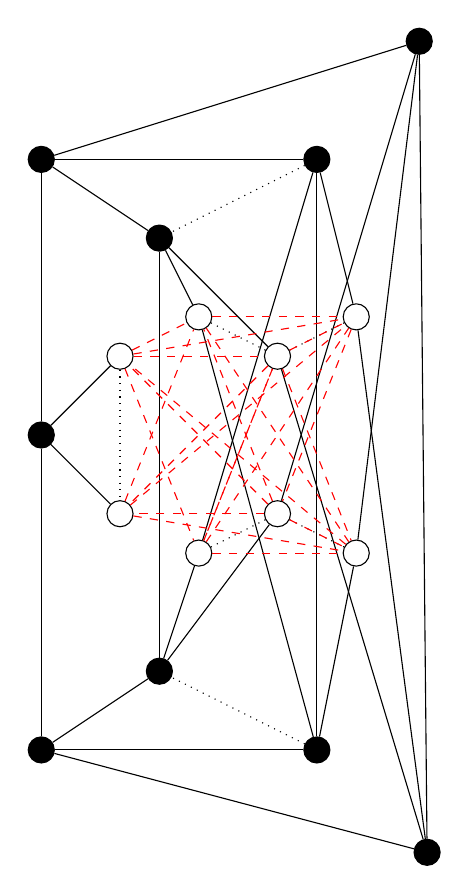
\begin{tikzpicture}
\node[circle,draw,fill] (v2) at (-2.5,4) {};
\node[circle,draw,fill] (v4) at (-1,3) {};
\node[circle,draw,fill] (v1) at (-2.5,0.5) {};
\node[circle,draw,fill] (v3) at (-2.5,-3.5) {};
\node[circle,draw,fill] (v7) at (-1,-2.5) {};
\node[circle,draw,fill] (v5) at (1,4) {};
\node[circle,draw,fill] (v6) at (2.3,5.5) {};
\node[circle,draw,fill] (v8) at (1,-3.5) {};
\node[circle,draw,fill] (v9) at (2.4,-4.8) {};

\draw  (v1) edge (v2);
\draw  (v1) edge (v3);
\draw  (v2) edge (v4);
\draw  (v2) edge (v5);
\draw  (v2) edge (v6);
\draw  (v3) edge (v7);
\draw  (v3) edge (v8);
\draw  (v3) edge (v9);
\draw  (v4) edge (v7);
\draw  (v5) edge (v8);
\draw  (v6) edge (v9);
\draw[dotted]  (v5) edge (v4);
\draw[dotted]  (v8) edge (v7);
\node[circle,draw] (v16) at (-1.5,1.5) {};
\node[circle,draw] (v17) at (-1.5,-0.5) {};
\draw  (v1) edge (v16);
\draw  (v1) edge (v17);

\node[draw,circle] (v10) at (-0.5,2) {};
\node[draw,circle] (v11) at (-0.5,-1) {};
\node[draw,circle] (v12) at (0.5,1.5) {};
\node[draw,circle] (v13) at (0.5,-0.5) {};
\node[draw,circle] (v15) at (1.5,-1) {};
\node[draw,circle] (v14) at (1.5,2) {};

\draw  (v4) edge (v10);
\draw  (v10) edge (v8);
\draw  (v7) edge (v11);
\draw  (v11) edge (v5);
\draw  (v4) edge (v12);
\draw  (v9) edge (v12);
\draw  (v7) edge (v13);
\draw  (v13) edge (v6);
\draw  (v5) edge (v14);
\draw  (v14) edge (v9);
\draw  (v8) edge (v15);
\draw  (v15) edge (v6);

\draw[dotted]  (v10) edge (v12);
\draw[dotted]  (v13) edge (v11);
\draw[dotted]  (v12) edge (v14);
\draw[dotted]  (v15) edge (v13);
\draw[dotted]  (v16) edge (v17);

\draw[dashed]  (v16) edge[red] (v10);
\draw[dashed]  (v16) edge[red] (v12);
\draw[dashed]  (v16) edge[red] (v14);
\draw[dashed]  (v13) edge[red] (v16);
\draw[dashed]  (v15) edge[red] (v16);
\draw[dashed]  (v16) edge[red] (v11);
\draw[dashed]  (v17) edge[red] (v10);
\draw[dashed]  (v12) edge[red] (v17);
\draw[dashed]  (v13) edge[red] (v17);
\draw[dashed]  (v17) edge[red] (v15);
\draw[dashed]  (v17) edge[red] (v14);
\draw[dashed]  (v13) edge[red] (v10);
\draw[dashed]  (v10) edge[red] (v15);
\draw[dashed]  (v11) edge[red] (v12);
\draw[dashed]  (v12) edge[red] (v11);
\draw[dashed]  (v12) edge[red] (v15);
\draw[dashed]  (v14) edge[red] (v13);
\draw[dashed]  (v11) edge[red] (v14);
\draw[dashed]  (v10) edge[red] (v14);
\draw[dashed] (v11) edge[red] (v15);
\draw[dashed]  (v12) edge[red] (v14);
\draw[dashed]  (v13) edge[red] (v15);
\end{tikzpicture}
\end{turn}
\end{frame}


\subsection{Convexidade}
\begin{frame}
\frametitle{Implementações}
\framesubtitle{Algoritmos - Convexidade $P_3$}
\centering
\adjustbox{max width=\textwidth}{
    \begin{tabular}{l|l|l}
               & \textbf{Algoritmo}         & \textbf{Abordagem}  \\ \hline
    \multicolumn{1}{l|}{1} & NumeroEnvoltorio(G(V,E))   & Exponencial         \\ \hline
    \multicolumn{1}{l|}{2} & NumeroCaratheodory(G(V,E)) & Exponencial         \\ \hline
    \multicolumn{1}{l|}{3} & AproxNEnvoltoria(G(V,E))   & Aproximativo Guloso \\ \hline
    \multicolumn{1}{l|}{4} & AproxNCaratheodory(G(V,E)) & Aproximativo Guloso \\ %\hline
    \end{tabular}
}
\end{frame}


\begin{frame}
\frametitle{Implementações}
\framesubtitle{Definição}
  \begin{columns}[T]
    \begin{column}{.3\textwidth}
    \begin{algorithm}[H]
        \SetAlFnt{\tiny}
        \SetAlCapFnt{\small}
        \SetAlCapNameFnt{\small}
        \SetAlgoLined
        \DontPrintSemicolon
        \LinesNumbered
        \SetAlgoLined
        \BlankLine
        \Entrada{$G(V,E)$ e $S | S \subseteq V(G)$}
        \Saida{$S^\prime$, menor conjunto convexo contendo S}
        \BlankLine

        $fila \gets S$ \\
        $S^\prime \gets \emptyset$ \\
        $cont[1...|V|] \gets 0$\\
        \Enqto{$fila \ne \emptyset$}{
            $v \gets remover(fila)$\\
            $cont[v] \gets 2$\\
            $S^\prime  \gets S^\prime \cup \{v\}$\\
            \ParaCada{$w \in Adj[v]$}{
                \Se{($cont[w] = 1)$}{
                    $inserir(w, fila)$\\
                }
                $cont[w] \gets cont[w] + 1$\\
            }
        }
        \Retorna{$S^\prime$}    
        \caption{$H(G(V,E),S)$}
    \end{algorithm}
    \end{column}
    \begin{column}{.3\textwidth}
        \begin{algorithm}[H]
        \SetAlFnt{\tiny}
        \SetAlCapFnt{\small}
        \SetAlCapNameFnt{\small}
        \SetAlgoLined
        \DontPrintSemicolon
        \LinesNumbered
        \SetAlgoLined
        \BlankLine
        \Entrada{$G(V,E)$, $S \subseteq V(G)$}
        \Saida{Verdadeiro se $S$ é um conjunto de Carathéodory}
        \BlankLine
        $S^\prime \gets H(G(V,E),S)$ \\
        \ParaCada{$u \in S$}{
            $S^{\prime \prime} \gets H(G(V,E),S \setminus \{u\})$ \\
            $S^\prime \gets S^\prime \setminus S^{\prime \prime}$ \\
        }
        \Retorna{$S^\prime \ne \emptyset$} 
        \caption{$ConjCarat(G(V,E),S)$} 
    \end{algorithm}
    \end{column}
    \begin{column}{.3\textwidth}
        \begin{algorithm}[H]
            \SetAlFnt{\tiny}
            \SetAlCapFnt{\small}
            \SetAlCapNameFnt{\small}
            \SetAlgoLined
            \DontPrintSemicolon
            \LinesNumbered
            \SetAlgoLined
            \BlankLine
            \Entrada{$G(V,E)$, $S \subseteq V(G)$}
            \Saida{Verdadeiro se $H(S) = V(G)$}
            \BlankLine
            $S^\prime \gets H(G(V,E),S)$ \\
            \Retorna{$|S^\prime| = |V|$} 
        \caption{$ConjEnv(G(V,E),S)$}   
        \end{algorithm}
    \end{column}
  \end{columns}
\end{frame}

\begin{frame}
\frametitle{Implementações}
\framesubtitle{NumeroEnvoltorio(G(V,E))}
  \begin{columns}[T]
    \begin{column}{.5\textwidth}
    \begin{algorithm}[H]
        \caption{$NumeroEnvoltorio(G(V,E))$}
        \SetAlFnt{\tiny}
        \SetAlCapFnt{\small}
        \SetAlCapNameFnt{\small}
        \SetAlgoLined
        \DontPrintSemicolon
        \LinesNumbered
        \SetAlgoLined
        \BlankLine
        \Entrada{$G(V,E)$}
        \Saida{h(G)}
        \BlankLine
        $h \gets 0$\\
        $k \gets 2$\\
        \Enqto{$k \le |V(G)| \land h = 0$}{
            \Se{$ConjuntoEnvoltoriaK(G(V,E),k)$}{
                $h \gets k$\\
            }
            $k \gets k + 1$\\          
        }
        \Retorna{h}
     \end{algorithm}
    \end{column}
    \begin{column}{.5\textwidth}
        \begin{algorithm}[H]
            \caption{$ConjuntoEnvoltoriaK(G(V,E),k)$}
            \label{alg:busca-conjunto-envoltoria-p3}
            \SetAlFnt{\tiny}
            \SetAlCapFnt{\small}
            \SetAlCapNameFnt{\small}
            \SetAlgoLined
            \DontPrintSemicolon
            \LinesNumbered
            \SetAlgoLined
            \BlankLine
            \Entrada{$G(V,E)$, inteiro $k \ge 1$}
            \Saida{Verdadeiro se $G(V,E)$ tem um conjunto envoltório de tamanho k}
            \BlankLine
            \BlankLine
            $c_{nk} \gets \frac{n!}{k!(n-k)!}$\\
            \Para{i de 1 até $c_{nk}$}{
                $S \gets Combinacao(V, k, i)$\\
                \Se{$ConjuntoEnvoltoria(G(V,E),S)$}{
                    \Retorna{\textbf{verdadeiro}}
                } 
            }
            \Retorna{\textbf{falso}} 
        \end{algorithm}
    \end{column}
  \end{columns}
\end{frame}

\begin{frame}
\frametitle{Implementações}
\framesubtitle{NumeroCaratheodory(G(V,E))}
  \begin{columns}[T]
    \begin{column}{.5\textwidth}
    \begin{algorithm}[H]
        \label{alg:numero-caratheodory-p3}
        \SetAlFnt{\tiny}
        \SetAlCapFnt{\small}
        \SetAlCapNameFnt{\small}
        \SetAlgoLined
        \DontPrintSemicolon
        \LinesNumbered
        \SetAlgoLined
        \BlankLine
        \Entrada{$G(V,E)$}
        \Saida{$c(G)$}
        \BlankLine
        $c \gets 0$\\
        $k \gets \frac{n + 1}{2}$\\
        \Enqto{$k \ge 1 \land c = 0$}{
            \Se{$ConjuntoCaratheodoryK(G(V,E),k)$}{
                $c \gets k$\\
            }
            $k \gets k - 1$\\ 
        }
        \Retorna{c}
    \caption{$NumeroCaratheodory(G(V,E))$}
    \end{algorithm}
    \end{column}
    \begin{column}{.5\textwidth}
        \begin{algorithm}[H]
            \label{alg:busca-conjunto-caratheodory-p3}
            \SetAlFnt{\tiny}
            \SetAlCapFnt{\small}
            \SetAlCapNameFnt{\small}
            \SetAlgoLined
            \DontPrintSemicolon
            \LinesNumbered
            \SetAlgoLined
            \BlankLine
            \Entrada{$G(V,E)$, inteiro $k \ge 1$}
            \Saida{Verdadeiro, se o grafo $G(V,E)$ tem um conjunto de Carathéodory de tamanho k}
            \BlankLine
            $c_{nk} \gets \frac{n!}{k!(n-k)!}$\\
            \Para{i de 1 até $c_{nk}$}{
                $S \gets Combinacao(V, k, i)$\\
                \Se{$ConjuntoCaratheodory(G(V,E),S)$}{
                    \Retorna{\textbf{verdadeiro}}
                } 
            }
            \Retorna{\textbf{falso}} 
            \caption{$ConjuntoCaratheodoryK(G(V,E),k)$}
        \end{algorithm}
    \end{column}
  \end{columns}
\end{frame}

\begin{frame}
\frametitle{Implementações}
\framesubtitle{Kernel Paralelo}
  \begin{columns}[T]
    \begin{column}{.5\textwidth}
    \begin{algorithm}[H]
        \SetAlFnt{\tiny}
        \SetAlCapFnt{\small}
        \SetAlCapNameFnt{\small}
        \SetAlgoLined
        \DontPrintSemicolon
        \LinesNumbered
        \SetAlgoLined
        \Entrada{$G(V,E), C_{nk}, k, \Delta$}
        \Saida{Envoltória $P_3$ Convexa}
        \Inicio{
            $id \gets Thread.Idx$\\
            $S \gets {\emptyset}$\\
            $H_{sp3} \gets{\emptyset}$\\
            $k \gets 1$\\
            $n \gets |V|$\\
            $n_{P3} \gets 0$\\
            $inicio \gets id * \Delta$\\
            $fim \gets (id+1) * \Delta$\\

            $S \gets Combinação(V, k, inicio)$\\
            \Para{(i de inicio até fim) $\land$ ($|H_{sp3}| < n$)}{
                $H_{sp3} \gets FuncaoHSP3(S, G(V,E))$\\
                $H_{sp3} \gets S \cup H_{sp3}$\\
                $S \gets ProximaCombinacao(S, V, k)$\\
            }
            \Retorna{$H_{sp3}$}
        }
        \caption{kernelNEnvoltoria}
    \end{algorithm}
    \end{column}
    \begin{column}{.5\textwidth}
        \begin{algorithm}[H]
        \SetAlFnt{\tiny}
        \SetAlCapFnt{\small}
        \SetAlCapNameFnt{\small}
        \SetAlgoLined
        \DontPrintSemicolon
        \LinesNumbered
        \Entrada{$G(V,E), C_{nk}, k, \Delta$}
        \Saida{Envoltória $P_3$ Convexa}
        \BlankLine
        \BlankLine
        \Inicio{
            $id \gets Thread.Idx$\\
            $S \gets {\emptyset}$\\
            $n \gets |V|$\\
            $\partial H_{sp3}\gets{\emptyset}$ \\
            $inicio \gets id * \Delta$\\
            $fim \gets (id+1) * \Delta$\\

            $S \gets Combinação(V, k, inicio)$\\
            \Para{($i$ de $inicio$ $fim$) $\land$ ($\partial H_{sp3}=\emptyset$)}{
                $\partial H_{sp3} \gets H(S) \backslash \cup _{p \in S} H(S \backslash \{p\}) $\\
                $S \gets ProximaCombinacao(S, V, i)$\\
            }
            \Retorna{$\partial H_{sp3}$}
             \BlankLine
        }
        \caption{kernelNCaratheodory}
        \end{algorithm}
    \end{column}
  \end{columns}
\end{frame}

\begin{frame}
\frametitle{Implementações}
\framesubtitle{AproxNEnvoltoria(G(V,E))}
  \begin{columns}[T]
    \begin{column}{.5\textwidth}
    \begin{algorithm}[H]
        \label{alg:aproximativo-numero-envoltoria-p3}
        \SetAlFnt{\tiny}
        \SetAlCapFnt{\small}
        \SetAlCapNameFnt{\small}
        \SetAlgoLined
        \DontPrintSemicolon
        \LinesNumbered
        \SetAlgoLined
        \BlankLine
        \Entrada{grafo $G(V,E)$}
        \Saida{inteiro k, número envoltório aproximado de  $G(V,E)$}
        \BlankLine

        $nenv \gets \infty $\\
        \ParaCada{$v \in V(G)$}{
            $S^\prime \gets \{v\}$\\
            $S \gets ExpandirConjEnvoltorio(G(V,E),S^\prime)$\\
            $nenv \gets \min\{|S|,nenv\}$\\        
        }
        \Retorna{nenv}
        \caption{$AproximativoNEnvoltoria(G(V,E))$}
    \end{algorithm}
    \end{column}
    \begin{column}{.5\textwidth}
    \begin{algorithm}[H]
    \label{alg:aproximativo-numero-envoltoria-p3-expansao}
        \SetAlFnt{\tiny}
        \SetAlCapFnt{\small}
        \SetAlCapNameFnt{\small}
        \SetAlgoLined
        \DontPrintSemicolon
        \LinesNumbered
        \SetAlgoLined
        \BlankLine
        \Entrada{$G(V,E), S^\prime \subseteq V(G)$}
        \Saida{Conjunto envoltório $S^\prime$}
        \BlankLine
        \Enqto{
            $|H(G(V,E),S^\prime)| < |V(G)|$
        }{
            $ve \gets \emptyset$\\ 
            $maiorHs \gets ncve \gets 0$\\
            \ParaCada{$w \in V(G)-S^\prime$}{
                $S_{aux} \gets S^\prime \cup \{w\}$\\
                $tamHs \gets |H(G(V,E),S_{aux})|$\\
                \Se{$tamHs \ge maiorHs \land |Adj[w]| > ncve$}{
                    $v_e \gets w$\\
                    $maiorHs \gets tamHs$\\
                    $ncve \gets  |Adj[w]| $\\
                }
            }{$S^\prime \gets S^\prime \cup \{v_e\} $}
        }
        \Retorna{$S^\prime$}
    \caption{$ExpandirConjuntoEnvoltoria(G(V,E),S^\prime)$}
    \end{algorithm}
    \end{column}
  \end{columns}
\end{frame}



\begin{frame}
\frametitle{Execução}
\framesubtitle{AproxNEnvoltoria(G(V,E))}
  \begin{columns}[T]
    \begin{column}{.5\textwidth}
    \centering
    \resizebox{\textwidth}{!}{%
        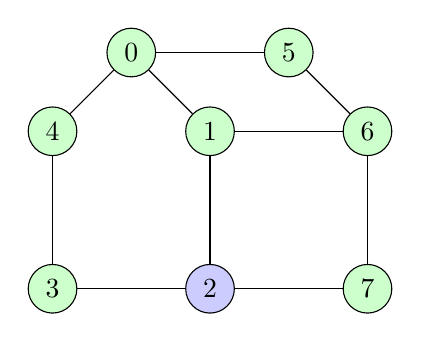
\begin{tikzpicture}[auto,node_style/.style={circle,draw=black,fill=green!20!},
           node_style_selected/.style={circle,draw=black,fill=red!20!},
           node_style_selected2/.style={circle,draw=black,fill=yellow!20!},
           node_style_selected3/.style={circle,draw=black,fill=blue!20!},
           edge_style/.style={draw=black}]
            \node[node_style] (v0) at (1, 3)  {0};
            \node[node_style] (v1) at (2, 2)  {1};
            \node[node_style_selected3] (v2) at (2, 0)  {2};
            \node[node_style] (v3) at (0, 0)  {3};
            \node[node_style] (v4) at (0, 2)  {4};
            \node[node_style] (v5) at (3, 3)  {5};
            \node[node_style] (v6) at (4, 2)  {6};
            \node[node_style] (v7) at (4, 0)  {7};
            \draw[edge_style]  (v0) edge node{} (v1);
            \draw[edge_style]  (v1) edge node{} (v2);
            \draw[edge_style]  (v2) edge node{} (v3);
            \draw[edge_style]  (v2) edge node{} (v7);
            \draw[edge_style]  (v3) edge node{} (v4);
            \draw[edge_style]  (v4) edge node{} (v0);
            \draw[edge_style]  (v0) edge node{} (v5);
            \draw[edge_style]  (v1) edge node{} (v6);
            \draw[edge_style]  (v5) edge node{} (v6);
            \draw[edge_style]  (v6) edge node{} (v7);
        \end{tikzpicture}
    }
    \end{column}
    \begin{column}{.5\textwidth}
     $S^\prime = \{\}$

     Melhor escolha gulosa: 2
    \end{column}
  \end{columns}
\end{frame}

\begin{frame}
\frametitle{Execução}
\framesubtitle{AproxNEnvoltoria(G(V,E))}
  \begin{columns}[T]
    \begin{column}{.5\textwidth}
    \centering
    \resizebox{\textwidth}{!}{%
        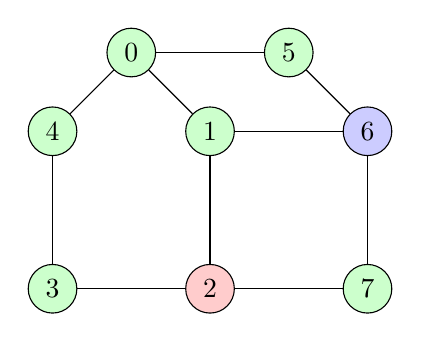
\begin{tikzpicture}[auto,node_style/.style={circle,draw=black,fill=green!20!},
           node_style_selected/.style={circle,draw=black,fill=red!20!},
           node_style_selected2/.style={circle,draw=black,fill=yellow!20!},
           node_style_selected3/.style={circle,draw=black,fill=blue!20!},
           edge_style/.style={draw=black}]
            \node[node_style] (v0) at (1, 3)  {0};
            \node[node_style] (v1) at (2, 2)  {1};
            \node[node_style_selected] (v2) at (2, 0)  {2};
            \node[node_style] (v3) at (0, 0)  {3};
            \node[node_style] (v4) at (0, 2)  {4};
            \node[node_style] (v5) at (3, 3)  {5};
            \node[node_style_selected3] (v6) at (4, 2)  {6};
            \node[node_style] (v7) at (4, 0)  {7};
            \draw[edge_style]  (v0) edge node{} (v1);
            \draw[edge_style]  (v1) edge node{} (v2);
            \draw[edge_style]  (v2) edge node{} (v3);
            \draw[edge_style]  (v2) edge node{} (v7);
            \draw[edge_style]  (v3) edge node{} (v4);
            \draw[edge_style]  (v4) edge node{} (v0);
            \draw[edge_style]  (v0) edge node{} (v5);
            \draw[edge_style]  (v1) edge node{} (v6);
            \draw[edge_style]  (v5) edge node{} (v6);
            \draw[edge_style]  (v6) edge node{} (v7);
        \end{tikzpicture}
    }
    \end{column}
    \begin{column}{.5\textwidth}
     $S^\prime = \{2\}$

     Melhor escolha gulosa: 6
    \end{column}
  \end{columns}
\end{frame}

\begin{frame}
\frametitle{Execução}
\framesubtitle{AproxNEnvoltoria(G(V,E))}
  \begin{columns}[T]
    \begin{column}{.5\textwidth}
    \centering
    \resizebox{\textwidth}{!}{%
        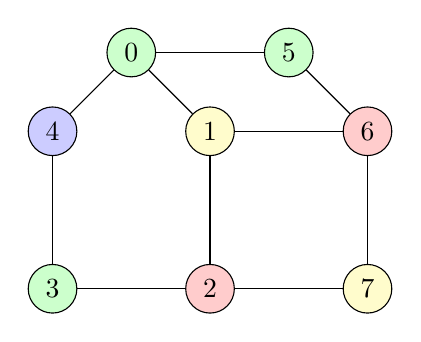
\begin{tikzpicture}[auto,node_style/.style={circle,draw=black,fill=green!20!},
           node_style_selected/.style={circle,draw=black,fill=red!20!},
           node_style_selected2/.style={circle,draw=black,fill=yellow!20!},
           node_style_selected3/.style={circle,draw=black,fill=blue!20!},
           edge_style/.style={draw=black}]
            \node[node_style] (v0) at (1, 3)  {0};
            \node[node_style_selected2] (v1) at (2, 2)  {1};
            \node[node_style_selected] (v2) at (2, 0)  {2};
            \node[node_style] (v3) at (0, 0)  {3};
            \node[node_style_selected3] (v4) at (0, 2)  {4};
            \node[node_style] (v5) at (3, 3)  {5};
            \node[node_style_selected] (v6) at (4, 2)  {6};
            \node[node_style_selected2] (v7) at (4, 0)  {7};
            \draw[edge_style]  (v0) edge node{} (v1);
            \draw[edge_style]  (v1) edge node{} (v2);
            \draw[edge_style]  (v2) edge node{} (v3);
            \draw[edge_style]  (v2) edge node{} (v7);
            \draw[edge_style]  (v3) edge node{} (v4);
            \draw[edge_style]  (v4) edge node{} (v0);
            \draw[edge_style]  (v0) edge node{} (v5);
            \draw[edge_style]  (v1) edge node{} (v6);
            \draw[edge_style]  (v5) edge node{} (v6);
            \draw[edge_style]  (v6) edge node{} (v7);
        \end{tikzpicture}
    }
    \end{column}
    \begin{column}{.5\textwidth}
     $S^\prime = \{2, 6\}$

     Melhor escolha gulosa: 4
    \end{column}
  \end{columns}
\end{frame}

\begin{frame}
\frametitle{Execução}
\framesubtitle{AproxNEnvoltoria(G(V,E))}
  \begin{columns}[T]
    \begin{column}{.5\textwidth}
    \centering
    \resizebox{\textwidth}{!}{%
        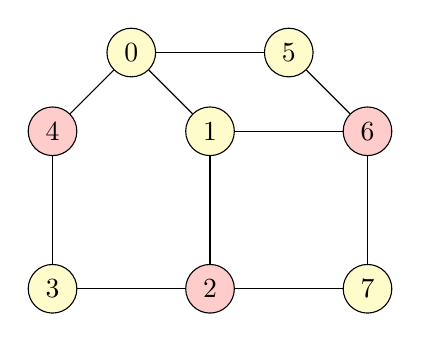
\begin{tikzpicture}[auto,node_style/.style={circle,draw=black,fill=green!20!},
           node_style_selected/.style={circle,draw=black,fill=red!20!},
           node_style_selected2/.style={circle,draw=black,fill=yellow!20!},
           node_style_selected3/.style={circle,draw=black,fill=blue!20!},
           edge_style/.style={draw=black}]
            \node[node_style_selected2] (v0) at (1, 3)  {0};
            \node[node_style_selected2] (v1) at (2, 2)  {1};
            \node[node_style_selected] (v2) at (2, 0)  {2};
            \node[node_style_selected2] (v3) at (0, 0)  {3};
            \node[node_style_selected] (v4) at (0, 2)  {4};
            \node[node_style_selected2] (v5) at (3, 3)  {5};
            \node[node_style_selected] (v6) at (4, 2)  {6};
            \node[node_style_selected2] (v7) at (4, 0)  {7};
            \draw[edge_style]  (v0) edge node{} (v1);
            \draw[edge_style]  (v1) edge node{} (v2);
            \draw[edge_style]  (v2) edge node{} (v3);
            \draw[edge_style]  (v2) edge node{} (v7);
            \draw[edge_style]  (v3) edge node{} (v4);
            \draw[edge_style]  (v4) edge node{} (v0);
            \draw[edge_style]  (v0) edge node{} (v5);
            \draw[edge_style]  (v1) edge node{} (v6);
            \draw[edge_style]  (v5) edge node{} (v6);
            \draw[edge_style]  (v6) edge node{} (v7);
        \end{tikzpicture}
    }
    \end{column}
    \begin{column}{.5\textwidth}
     $S^\prime = \{2, 6, 4\}$
    \end{column}
  \end{columns}
\end{frame}

\begin{frame}
\frametitle{Implementações}
\framesubtitle{AproxNCaratheodory(G(V,E))}
\begin{columns}[T]
\begin{column}{.6\textwidth}
\begin{algorithm}[H]
    \label{alg:aproximativo-numero-caratheodory-p3}
    \SetAlFnt{\tiny}
    \SetAlCapFnt{\small}
    \SetAlCapNameFnt{\small}
    \SetAlgoLined
    \DontPrintSemicolon
    \LinesNumbered
    \SetAlgoLined
    \BlankLine
    \Entrada{$G(V,E)$}
    \Saida{inteiro k, número aproximado de Carathéodoryo de  $G(V,E)$}
    \BlankLine
    $c \gets 0$\\
    \ParaCada{$v \in V(G)||Adj[v]| \ge 2$}{
        $S \gets ConstroiConjCaratheodoryDoParcial(G(V,E),v)$\\
        $S \gets ExpandirConjuntoCaratheodory(G(V,E),S)$\\
        $c \gets \max\{|S|,ncarat\}$\\        
    }
    \Retorna{c}
    \caption{$AproximativoNCaratheodory(G(V,E))$}
\end{algorithm}
\end{column}
\end{columns}
\end{frame}

\begin{frame}
\frametitle{Implementações}
\framesubtitle{AproxNCaratheodory(G(V,E))}
  \begin{columns}[T]
    \begin{column}{.5\textwidth}
        \begin{algorithm}[H]
            \label{alg:aproximativo-numero-caratheodory-p3-parcial}
            \SetAlFnt{\tiny}
            \SetAlCapFnt{\small}
            \SetAlCapNameFnt{\small}
            \SetAlgoLined
            \DontPrintSemicolon
            \LinesNumbered
            \SetAlgoLined
            \BlankLine
            \Entrada{$G(V,E)$}
            \BlankLine            
            \Entrada{vértice $v \in V(G) | |Adj[v]| \ge 2$}
            \BlankLine            
            \Saida{conjunto de Caratheodory $S$}
            \BlankLine
            \BlankLine
            $S \gets \{v\}$\\
            $fila \gets S$ \\
            \Enqto{
                $fila \ne \emptyset$
            }{
                $v_p \gets remover(fila)$\\
                $S^\prime \gets Adj2MenorGrau[v_p,S\cup\{v\}]$\\
                $S_{aux} \gets S^\prime \cup S \setminus \{v_p\} $\\
                \Se{$ConjuntoCaratheodory(G(V,E),S_{aux})$}{
                    $inserir(S^\prime, fila)$\\
                    $S \gets S_{aux}$\\
                }
            }
            \Retorna{S}
            \caption{$ConjCaratDoParcial(G(V,E),v)$}       
        \end{algorithm}
    \end{column}
    \begin{column}{.5\textwidth}
    \begin{algorithm}[H]
        \label{alg:aproximativo-numero-caratheodory-p3-expansao}
        \SetAlFnt{\tiny}
        \SetAlCapFnt{\small}
        \SetAlCapNameFnt{\small}
        \SetAlgoLined
        \DontPrintSemicolon
        \LinesNumbered
        \SetAlgoLined
        \BlankLine

        \Entrada{$G(V,E)$ e vértice $v \in V(G)$}

        \Saida{conjunto de Caratheodory S otimizado}
        \BlankLine
        \Repita{
            $V_e \ne \emptyset $
        }{
            $Ve \gets \emptyset$\\
            $t_{hsve} \gets \infty$\\
            \ParaCada{$v \in V(G) \setminus S$}{
                $S_{aux} \gets S \cup \{v\}$\\
                $cc \gets ConjuntoCaratheodory(G(V,E),S_{aux})$
                $t_{hs} \gets |H(G(V,E),S_{aux})|$\\
                \Se{$cc \land (t_{hsve} =  \infty \lor (t_{hs} \le t_{hsve} \land |Adj[v]| < |Adj[v_e]|))$}{
                    $V_e \gets \{v\}$\\
                    $t_{hsve} \gets t_{hs}$\\
                }
            }{$S \gets S \cup \{V_e\} $}
        }
        \Retorna{S}
    \caption{$ExpandirConjCarat(G(V,E),S)$}
    \end{algorithm}
    \end{column}
  \end{columns}
\end{frame}


\begin{frame}
\frametitle{Execução}
\framesubtitle{AproxNCaratheodory(G(V,E))}
 \begin{columns}[T]
    \begin{column}{.5\textwidth}
    \centering
    \resizebox{\textwidth}{!}{%
        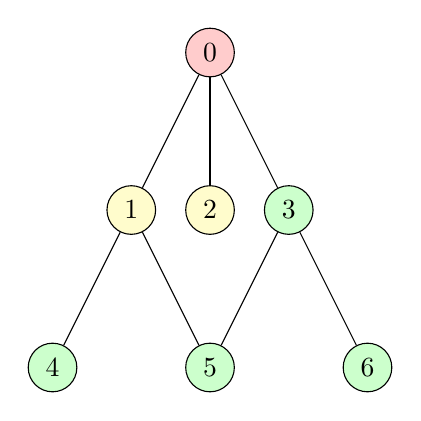
\begin{tikzpicture}
        [auto,
         node_style/.style={circle,draw=black,fill=green!20!},
         node_style_selected/.style={circle,draw=black,fill=red!20!},
         node_style_selected2/.style={circle,draw=black,fill=yellow!20!},
         node_style_selected3/.style={circle,draw=black,fill=blue!20!},
         edge_style/.style={draw=black}]
            \node[node_style_selected] (v0) at (2, 4)  {0};
            \node[node_style_selected2] (v1) at (1, 2)  {1};
            \node[node_style_selected2] (v2) at (2, 2)  {2};
            \node[node_style] (v3) at (3, 2)  {3};
            \node[node_style] (v4) at (0, 0)  {4};
            \node[node_style] (v5) at (2, 0)  {5};
            \node[node_style] (v6) at (4, 0)  {6};
            \draw[edge_style]  (v0) edge node{} (v1);
            \draw[edge_style]  (v0) edge node{} (v2);
            \draw[edge_style]  (v0) edge node{} (v3);
            \draw[edge_style]  (v1) edge node{} (v4);
            \draw[edge_style]  (v1) edge node{} (v5);
            \draw[edge_style]  (v3) edge node{} (v5);
            \draw[edge_style]  (v3) edge node{} (v6);
        \end{tikzpicture}%
    }
    \end{column}
    \begin{column}{.5\textwidth}
        $S=\{0\}$\\
        $v_p=0$\\
        $S^\prime=\{1, 2\}$\\
        $S_{aux}=\{1, 2\}$\\
        $fila = 0 $        
    \end{column}
  \end{columns}
\end{frame}

\begin{frame}
\frametitle{Execução}
\framesubtitle{AproxNCaratheodory(G(V,E))}
 \begin{columns}[T]
    \begin{column}{.5\textwidth}
    \centering
    \resizebox{\textwidth}{!}{%
        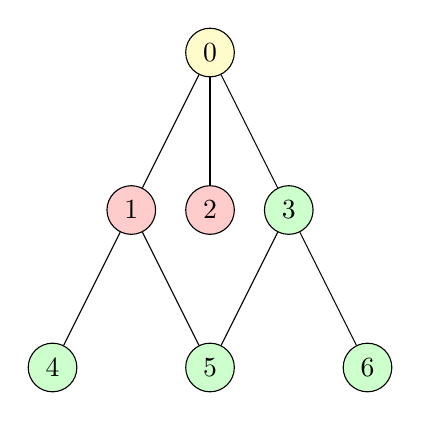
\begin{tikzpicture}
        [auto,
         node_style/.style={circle,draw=black,fill=green!20!},
         node_style_selected/.style={circle,draw=black,fill=red!20!},
         node_style_selected2/.style={circle,draw=black,fill=yellow!20!},
         node_style_selected3/.style={circle,draw=black,fill=blue!20!},
         edge_style/.style={draw=black}]
            \node[node_style_selected2] (v0) at (2, 4)  {0};
            \node[node_style_selected] (v1) at (1, 2)  {1};
            \node[node_style_selected] (v2) at (2, 2)  {2};
            \node[node_style] (v3) at (3, 2)  {3};
            \node[node_style] (v4) at (0, 0)  {4};
            \node[node_style] (v5) at (2, 0)  {5};
            \node[node_style] (v6) at (4, 0)  {6};
            \draw[edge_style]  (v0) edge node{} (v1);
            \draw[edge_style]  (v0) edge node{} (v2);
            \draw[edge_style]  (v0) edge node{} (v3);
            \draw[edge_style]  (v1) edge node{} (v4);
            \draw[edge_style]  (v1) edge node{} (v5);
            \draw[edge_style]  (v3) edge node{} (v5);
            \draw[edge_style]  (v3) edge node{} (v6);
        \end{tikzpicture}%
    }
    \end{column}
    \begin{column}{.5\textwidth}
        $S=\{1,2\}$\\
        $v_p=1$\\
        $S^\prime=\{4, 5\}$\\
        $S_{aux}=\{2,4,5\}$\\
        $fila = \{1,2\} $        
    \end{column}
  \end{columns}
\end{frame}


\begin{frame}
\frametitle{Execução}
\framesubtitle{AproxNCaratheodory(G(V,E))}
 \begin{columns}[T]
    \begin{column}{.5\textwidth}
    \centering
    \resizebox{\textwidth}{!}{%
        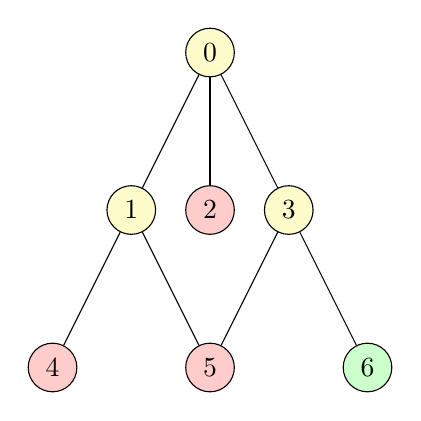
\begin{tikzpicture}
        [auto,
         node_style/.style={circle,draw=black,fill=green!20!},
         node_style_selected/.style={circle,draw=black,fill=red!20!},
         node_style_selected2/.style={circle,draw=black,fill=yellow!20!},
         node_style_selected3/.style={circle,draw=black,fill=blue!20!},
         edge_style/.style={draw=black}]
            \node[node_style_selected2] (v0) at (2, 4)  {0};
            \node[node_style_selected2] (v1) at (1, 2)  {1};
            \node[node_style_selected] (v2) at (2, 2)  {2};
            \node[node_style_selected2] (v3) at (3, 2)  {3};
            \node[node_style_selected] (v4) at (0, 0)  {4};
            \node[node_style_selected] (v5) at (2, 0)  {5};
            \node[node_style] (v6) at (4, 0)  {6};
            \draw[edge_style]  (v0) edge node{} (v1);
            \draw[edge_style]  (v0) edge node{} (v2);
            \draw[edge_style]  (v0) edge node{} (v3);
            \draw[edge_style]  (v1) edge node{} (v4);
            \draw[edge_style]  (v1) edge node{} (v5);
            \draw[edge_style]  (v3) edge node{} (v5);
            \draw[edge_style]  (v3) edge node{} (v6);
        \end{tikzpicture}%
    }
    \end{column}
    \begin{column}{.5\textwidth}
        $S=\{2,4,5\}$\\
        $v_p=2$\\
        $S^\prime=\emptyset$\\
        $S_{aux}=\{2,4,5\}$\\
        $fila = \{2,4,5\} $        
    \end{column}
  \end{columns}
\end{frame}

\begin{frame}
\frametitle{Execução}
\framesubtitle{AproxNCaratheodory(G(V,E))}
 \begin{columns}[T]
    \begin{column}{.5\textwidth}
    \centering
    \resizebox{\textwidth}{!}{%
        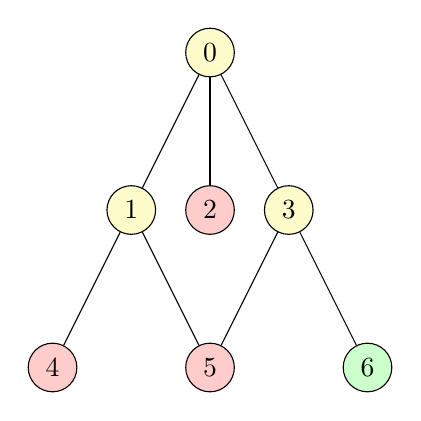
\begin{tikzpicture}
        [auto,
         node_style/.style={circle,draw=black,fill=green!20!},
         node_style_selected/.style={circle,draw=black,fill=red!20!},
         node_style_selected2/.style={circle,draw=black,fill=yellow!20!},
         node_style_selected3/.style={circle,draw=black,fill=blue!20!},
         edge_style/.style={draw=black}]
            \node[node_style_selected2] (v0) at (2, 4)  {0};
            \node[node_style_selected2] (v1) at (1, 2)  {1};
            \node[node_style_selected] (v2) at (2, 2)  {2};
            \node[node_style_selected2] (v3) at (3, 2)  {3};
            \node[node_style_selected] (v4) at (0, 0)  {4};
            \node[node_style_selected] (v5) at (2, 0)  {5};
            \node[node_style] (v6) at (4, 0)  {6};
            \draw[edge_style]  (v0) edge node{} (v1);
            \draw[edge_style]  (v0) edge node{} (v2);
            \draw[edge_style]  (v0) edge node{} (v3);
            \draw[edge_style]  (v1) edge node{} (v4);
            \draw[edge_style]  (v1) edge node{} (v5);
            \draw[edge_style]  (v3) edge node{} (v5);
            \draw[edge_style]  (v3) edge node{} (v6);
        \end{tikzpicture}%
    }
    \end{column}
    \begin{column}{.5\textwidth}
        $S=\{2,4,5\}$\\
        $v_p=4$\\
        $S^\prime=\emptyset$\\
        $S_{aux}=\{2,4,5\}$\\
        $fila = \{4,5\} $        
    \end{column}
  \end{columns}
\end{frame}

\begin{frame}
\frametitle{Execução}
\framesubtitle{AproxNCaratheodory(G(V,E))}
 \begin{columns}[T]
    \begin{column}{.5\textwidth}
    \centering
    \resizebox{\textwidth}{!}{%
        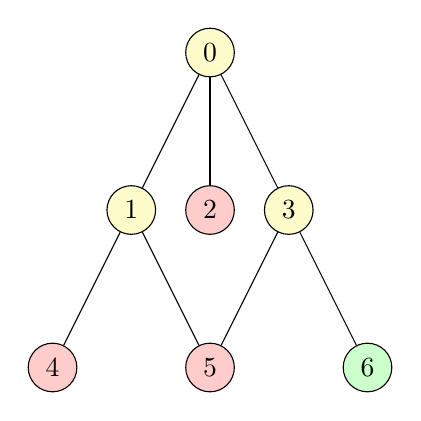
\begin{tikzpicture}
        [auto,
         node_style/.style={circle,draw=black,fill=green!20!},
         node_style_selected/.style={circle,draw=black,fill=red!20!},
         node_style_selected2/.style={circle,draw=black,fill=yellow!20!},
         node_style_selected3/.style={circle,draw=black,fill=blue!20!},
         edge_style/.style={draw=black}]
            \node[node_style_selected2] (v0) at (2, 4)  {0};
            \node[node_style_selected2] (v1) at (1, 2)  {1};
            \node[node_style_selected] (v2) at (2, 2)  {2};
            \node[node_style_selected2] (v3) at (3, 2)  {3};
            \node[node_style_selected] (v4) at (0, 0)  {4};
            \node[node_style_selected] (v5) at (2, 0)  {5};
            \node[node_style] (v6) at (4, 0)  {6};
            \draw[edge_style]  (v0) edge node{} (v1);
            \draw[edge_style]  (v0) edge node{} (v2);
            \draw[edge_style]  (v0) edge node{} (v3);
            \draw[edge_style]  (v1) edge node{} (v4);
            \draw[edge_style]  (v1) edge node{} (v5);
            \draw[edge_style]  (v3) edge node{} (v5);
            \draw[edge_style]  (v3) edge node{} (v6);
        \end{tikzpicture}%
    }
    \end{column}
    \begin{column}{.5\textwidth}
        $S=\{2,4,5\}$\\
        $v_p=5$\\
        $S^\prime=\emptyset$\\
        $S_{aux}=\{2,4,5\}$\\
        $fila = \{5\} $        
    \end{column}
  \end{columns}
\end{frame}


\begin{frame}
\frametitle{Execução}
\framesubtitle{AproxNCaratheodory(G(V,E))}
 \begin{columns}[T]
    \begin{column}{.5\textwidth}
    \centering
    \resizebox{\textwidth}{!}{%
        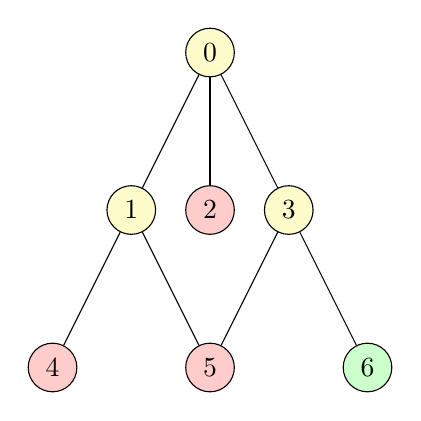
\begin{tikzpicture}
        [auto,
         node_style/.style={circle,draw=black,fill=green!20!},
         node_style_selected/.style={circle,draw=black,fill=red!20!},
         node_style_selected2/.style={circle,draw=black,fill=yellow!20!},
         node_style_selected3/.style={circle,draw=black,fill=blue!20!},
         edge_style/.style={draw=black}]
            \node[node_style_selected2] (v0) at (2, 4)  {0};
            \node[node_style_selected2] (v1) at (1, 2)  {1};
            \node[node_style_selected] (v2) at (2, 2)  {2};
            \node[node_style_selected2] (v3) at (3, 2)  {3};
            \node[node_style_selected] (v4) at (0, 0)  {4};
            \node[node_style_selected] (v5) at (2, 0)  {5};
            \node[node_style] (v6) at (4, 0)  {6};
            \draw[edge_style]  (v0) edge node{} (v1);
            \draw[edge_style]  (v0) edge node{} (v2);
            \draw[edge_style]  (v0) edge node{} (v3);
            \draw[edge_style]  (v1) edge node{} (v4);
            \draw[edge_style]  (v1) edge node{} (v5);
            \draw[edge_style]  (v3) edge node{} (v5);
            \draw[edge_style]  (v3) edge node{} (v6);
        \end{tikzpicture}%
    }
    \end{column}
    \begin{column}{.5\textwidth}
        $S=\{2,4,5\}$\\

        Expandir S? Não
    \end{column}
  \end{columns}
\end{frame}

\begin{frame}
\frametitle{Resultados Execução}
%\framesubtitle{Execução}
\centering
\adjustbox{max width=.8\textwidth}{
    \begin{tabular}{r|r|r|r}
    \textbf{Classe Grafos}    & \textbf{\begin{tabular}[c]{@{}l@{}}Extensão\\ de Vértices\end{tabular}}
                              & \textbf{\begin{tabular}[c]{@{}l@{}}Quantidade\\Carathéodory\end{tabular}}
                              & \textbf{\begin{tabular}[c]{@{}l@{}}Quantidade\\Envoltório\end{tabular}} \\ \hline
    Hipo-hamiltoniano         & 10-24       & 3.379        & 3.379      \\ \hline
    Quase hipo-hamiltoniano   & 17-32       & 688          & 831        \\ \hline
    Crítico sem H             & 4-16        & 1.041        & 1.041      \\ \hline
    Maximal sem triangulo     & 3-30        & 1.536.047    & 1.536.047  \\ \hline
    Fortemente regular        & 25-40       & 43.669       & 43.669     \\ \hline
    Cúbico                    & 4-32        & 241.705      & 3.964.513  \\ \hline
    Quártico                  & 5-37        & 122.583      & 138.427    \\ \hline
    Snarks                    & 10-32       & 3.493        & 9.623      \\ \hline
    Vértice-transitivo        & 3-31        & 19.260       & 37.477     \\ \hline
    Minimal Ramsey(3,k)       & 16-35       & 6.972        & 76.697     \\ \hline
    Nº de Ramsey R(K3,G)      & 10-36       & 1.628.788    & 1.628.788  \\ \hline
    Árvores                   & 3-20        & 874.321      & 874.321    \\ \hline
    \multicolumn{2}{r|}{\textbf{Total:}} & \textbf{4.481.946}   & \multicolumn{1}{l}{\textbf{8.314.813}} \\
    \multicolumn{2}{r|}{\textbf{Tempo força bruta:}} & \textbf{240h}         & \multicolumn{1}{l}{\textbf{41h}} \\
    \multicolumn{2}{r|}{\textbf{Tempo aproximativo otimizado:}} & \textbf{17h}          & \multicolumn{1}{l}{\textbf{2h}} \\
    \end{tabular}
}
\end{frame}

\begin{frame}
\frametitle{Resultados Execução}
\framesubtitle{Soluções Aproximadas}
\centering
\begin{tabular}{r|r|r|r}
\textbf{Classe Grafos}    & \textbf{\begin{tabular}[c]{@{}l@{}}Extensão\\ de Vértices\end{tabular}}
      & \textbf{\begin{tabular}[c]{@{}l@{}}Aproximativo\\Carathéodory\end{tabular}}
      & \textbf{\begin{tabular}[c]{@{}l@{}}Aproximativo\\Envoltório\end{tabular}} \\ \hline
Crítico sem H         & 4-16  & \begin{tabular}[r]{@{}r@{}}1.041\\$(>90\%)$\end{tabular} & \begin{tabular}[r]{@{}r@{}}1.041\\$(>90\%)$\end{tabular}      \\ \hline
Maximal sem triangulo & 3-30  & \begin{tabular}[r]{@{}r@{}}1.536.047\\$(>90\%)$\end{tabular} & \begin{tabular}[r]{@{}r@{}}1.536.047\\$(>90\%)$\end{tabular} \\ \hline
Fortemente regular    & 25-40 & \begin{tabular}[r]{@{}r@{}}43.669\\ $(100\%)$\end{tabular}         &  \begin{tabular}[r]{@{}r@{}}43.669\\ $(100\%)$\end{tabular} \\ \hline
Quártico              & 5-37  & \begin{tabular}[r]{@{}r@{}}122.583\\ $(>70\%)$\end{tabular}  & \begin{tabular}[r]{@{}r@{}}138.427\\ $(>70\%)$\end{tabular} \\ \hline
Snarks                & 10-32 & \begin{tabular}[r]{@{}r@{}}3.493\\ $(>80\%)$\end{tabular}  & \begin{tabular}[r]{@{}r@{}}9.623\\ $(>80\%)$\end{tabular}      \\ \hline
Vértice-transitivo    & 3-31  & 19.260 (--)      & 37.477  $(>95\%)$      \\
\end{tabular}
\end{frame}


% \begin{frame}
% \frametitle{Aproximativo Envoltório}
% \framesubtitle{Melhorias Finais}
%     Forma de Entrada:
%     \begin{itemize}
%      \item Poucos grafos grandes;
%      \item Muitos grafos pequenos e médios;     
%     \end{itemize}
    
%     Estrategias de paralelização:
%         \begin{itemize}
%       \item Um grafo por Thread;
%       \item Um grafo por Bloco;     
%       \item Um grafo por Grid;  
%     \end{itemize}
% \end{frame}

% \begin{frame}
% \frametitle{Otimização do Aproximativo Envoltório}
% \framesubtitle{Entrada}
%  \begin{columns}[T]
%     \begin{column}{.5\textwidth}
%     \centering
%     \resizebox{\textwidth}{!}{%
%         \centering
%         \includegraphics[scale=.5]{img/csr-exemplo.png}
%     }
%     \end{column}
%     \begin{column}{.5\textwidth}
%         Tipo de Entradas interessantes ao problema:
%         \begin{itemize}
%          \item Muitos grafos pequenos e médios; 
%          %\item Quantidade de vértices heterogênea;     
%         \end{itemize}
    
%         Estrutura de dados empregada individualmente:
%         \begin{itemize}
%             \item{Matriz de Adjacência Compacta - CSR}
%             \item{Concatenar todas as Listas de Adjacência em um Vetor C}
%             \item{Um vetor auxiliar com índice de inicio de cada lista}
%         \end{itemize}
%     \end{column}
%   \end{columns}
% \end{frame}


% \begin{frame}
% \frametitle{Formato de Entrada}
% \framesubtitle{Entrada Múltipla}
%  \begin{columns}[T]
%     \begin{column}{.5\textwidth}
%     \centering
%     \resizebox{\textwidth}{!}{%
%         \centering
%         \includegraphics[scale=.5]{img/3-1.png}
%     }
%     \end{column}
%     \begin{column}{.5\textwidth}    
%         Estrutura de dados empregada para múltiplos:
%         \begin{itemize}
%             \item{Matriz de Adjacência Compacta - CSR}
%             \item{Concatenar todos os grafos em um vetor Gs}
%             \item{Um vetor I auxiliar com índice de inicio de cada grafo}
%         \end{itemize}
%     \end{column}
%   \end{columns}
% \end{frame}



% \begin{frame}
% \frametitle{Aproximativo Envoltório}
% \framesubtitle{Testes iniciais de estratégia de paralelismo}
%     Estratégias de divisão de trabalho testadas:
%     \begin{itemize}
%      \item Um grafo por Thread
%      \item Um grafo por Bloco
%      \item Um grafo por Grid
%      \item Um grafo por Hibrida Bloco-Grid
%     \end{itemize}
% \end{frame}


% \begin{frame}
% \frametitle{Teste}
% \framesubtitle{Grafo/Thread}
%  \begin{columns}[T]
%     \begin{column}{.5\textwidth}
%          \begin{itemize}
%          \item Baixa ocupação
%          \item Carga de trabalho das Threads altamente desbalanceada
%          \item Speedup < 0
%          \end{itemize}
%     \end{column}
%     \begin{column}{.5\textwidth}

%     \end{column}
%   \end{columns}
% \end{frame}

% \begin{frame}
% \frametitle{Teste}
% \framesubtitle{Grafo/Bloco}
%  \begin{columns}[T]
%     \begin{column}{.5\textwidth}
%          \begin{itemize}
%          \item Melhor ocupação;
%          \item Carga de trabalho mais balanceada;     
%          \item Speedup $3\sim 4x$;              
%          \item Dificuldade: Balanceamento de carga de trabalho entre os blocos;
%          \item  $n_t \gets max(|V(G)|)$;
%          \item $n_t\gets k\times$WARP\_SIZE;
%          \item Quase sempre $|V(G)| mod n_t$ > 0;
%          \end{itemize}
%     \end{column}
%     \begin{column}{.5\textwidth}
%     \resizebox{\textwidth}{!}{%
%         \centering
%         \includegraphics[scale=.5]{img/nvvp-abordagem-b.png}
%     }
%     \end{column}
%   \end{columns}
% \end{frame}

% \begin{frame}
% \frametitle{Teste}
% \framesubtitle{Grafo/Grid/Stream}
%  \begin{columns}[T]
%     \begin{column}{.5\textwidth}
%     \resizebox{\textwidth}{!}{%
%         \centering
%         \includegraphics[scale=.5]{img/nvvp-abordagem-x.png}
%     }
%     \end{column}
%     \begin{column}{.5\textwidth}
%          \begin{itemize}
%          \item Melhor ocupação;
%          \item Stream (não bloqueantes) separadas;
%          \item Carga de trabalho mais balanceada entre Threads e blocos;     
%          \item Speedup $4\sim 5x$;              
%          \item Algumas Grids sub-utilizadas;
%          \item Se $|V(G)|<$WARP\_SIZE;
%          \end{itemize}
%     \end{column}
%   \end{columns}
% \end{frame}

% \begin{frame}
% \frametitle{Teste}
% \framesubtitle{Combinação da Abordagem Bloco e Grid}
%  \begin{columns}[T]
%     \begin{column}{.5\textwidth}
%     \resizebox{\textwidth}{!}{%
%         \centering
%         \includegraphics[scale=.5]{img/nvv-abordagem-o.png}
%     }
%     \end{column}
%     \begin{column}{.5\textwidth}
%          \begin{itemize}
%          \item Melhor ocupação;
%          \item Kernel para Grafos com $|V(G)|$ múltiplos de WARP\_SIZE;
%          \item Kernel que agrupe o trabalho "truncado" em blocos com quantidade de threads multiplos de WARP\_SIZE;     
%          \item Speedup $5 \sim 7x$;              
%          \item Se $|V(G)|<$WARP\_SIZE algumas Grids podem estar sub-utilizadas;
%          \end{itemize}
%     \end{column}
%   \end{columns}
% \end{frame}

% \begin{frame}
% \frametitle{Teste}
% \framesubtitle{Algoritmo Combinação da Abordagem Bloco e Grid}
% \framesubtitle{Combinação da Abordagem Bloco e Grid}
% \begin{columns}[T]
% \begin{column}{.7\textwidth}
% \begin{algorithm}[H]
% \SetAlFnt{\tiny}
% \SetAlCapFnt{\small}
% \SetAlCapNameFnt{\small}
% \SetAlgoLined
% \Entrada{$G_s$}
% \Saida{Envoltória Aproximada de $G_s$}
% \Inicio{
% %    for (int i = 0; i < cont; i++) {
% %            graphCsr *graph = &graphs[i];
% %            int nvertice = graph->data[0];
% %            if (nvertice >= BLOCK_WINDOWS) {
% %                nblocksoptimal++;
% %            }
% %            int vertrunk = nvertice % BLOCK_WINDOWS;
% %            nvertstrunk = nvertstrunk + vertrunk;
% %      }

% $ R_s \gets \emptyset $\\
% $ M_w \gets \emptyset $\\
% $ nblk \gets 0 $\\

% \ParaCada{$g \in G_s$}{
%   $n \gets |V(g)|$ \\
%   $R_s[g] \gets n $\\
%   \Se{$n \ge TAMBLOCK $}{
%     $nblk \gets nblk + 1$\\
%   }
%   $nvtrunc \gets n$ {\bf mod} $TAMBLOCK $\\
%   $tntrunc \gets tntrunc + vtrunk $\\        
%   \Para{$i$ de $1$ até $nvtrunc$}{
% 	$v \gets \frac{n}{TAMBLOCK} \times TAMBLOCK + i$ \\
% 	$ M_w.add(\{g,v\})$\\
%   }
% }
% $nblktrunc \gets \frac{nvertstrunk}{TAMBLOCKTRUNC}$\\
% $kernelAproxEnvoltGrafBlk<<<nblk, TAMBLOCK>>>(G_s, R_s)$\\
% $kernelAproxEnvGrafBlkTrunc<<<nblktrunc, TAMBLOCKTRUNC>>>(G_s, R_s, M_w, tntrunc)$\\
% \Retorna{$R_s$}
% }
% \label{alg-aproximativo-abordagem-hibrida}
% \caption{AlgoritmoAproxCombEnv}
% \end{algorithm}
% \end{column}
% \end{columns}
% \end{frame}


% \begin{frame}
% \frametitle{Teste}
% \framesubtitle{Kernel Algoritmo Combinação da Abordagem Bloco e Grid}
% \begin{columns}[T]
% \begin{column}{.5\textwidth}
% \begin{algorithm}[H]
% \SetAlFnt{\tiny}
%         \SetAlCapFnt{\small}
%         \SetAlCapNameFnt{\small}
%         \SetAlgoLined
%         \Entrada{$G_s$}
%         \Saida{Nº Envoltório Aproximado $R_s$ }
		
%             $shared$ $rlocal$\\			
% 			\Se{$threadIdx = 0$}{
%             	$rlocal \gets \infty$\\
%             }
%             $syncthreads()$\\
%         	$g \gets G_s[blockIdx]$;  $i \gets 0$; $n \gets |V(g)|$; $id \gets threadIdx$\\        
%             \Enqto{
%             	$id < n$
%             }{
%             	$v \gets id$; $S^\prime \gets \{v\}$\\                                
%                 \Enqto{$|H(g,S^\prime)| < n$}{
%                     $ve \gets \emptyset$; $mHs \gets ncve \gets 0$\\
%                     \ParaCada{$w \in V(g)-S^\prime$}{
%                         $S_{aux} \gets S^\prime \cup \{w\}$; $tHs \gets |H(g,S_{aux})|$\\
%                         \Se{$tHs \ge mHs \land |Adj[w]| > ncve$}{
%                             $v_e \gets w$; $mHs \gets tHs$; $ncve \gets  |Adj[w]| $\\
%                         }
%                     }{$S^\prime \gets S^\prime \cup \{v_e\}$}
%                 }
                
%                 $i \gets i + 1$; $id \gets id + (i \times TAMBLOCK)$\\
%             }
% 			$syncthreads()$\\
%             \Se{$threadIdx = 0$}{
%             	$R_s[g]=rlocal$\\
%             }        
%         \caption{kernelAproxEnvoltGrafBlk}
% \end{algorithm}
% \end{column}
% \begin{column}{.5\textwidth}
% \begin{algorithm}[H]
%         \SetAlFnt{\tiny}
%         \SetAlCapFnt{\small}
%         \SetAlCapNameFnt{\small}
%         \SetAlgoLined
%         \Entrada{$G_s$, $M_w$, $tntrunc$}
%         \Saida{Nº Envoltório Aproximado $R_s$ }
        
%             $id \gets blockIdx + threadIdx$\\
%             $i \gets 0$\\
%             \Enqto{
%             	$id < tntrunc$
%             }{
%                 $g \gets M_w[id][0]$\\
%             	$v \gets M_w[id][1]$\\
%                 %exapandHullSetFromV\\
%                 $S^\prime \gets \{v\}$\\
%                 \Enqto{$|H(g,S^\prime)| < n$}{
%                     $ve \gets \emptyset$\\
%                     $mHs \gets ncve \gets 0$\\
%                     \ParaCada{$w \in V(g)-S^\prime$}{
%                         $S_{aux} \gets S^\prime \cup \{w\}$\\
%                         $tHs \gets |H(g,S_{aux})|$\\
%                         \Se{$tHs \ge mHs \land |Adj[w]| > ncve$}{
%                             $v_e \gets w$\\
%                             $mHs \gets tHs$\\
%                             $ncve \gets  |Adj[w]| $\\
%                         }
%                     }{$S^\prime \gets S^\prime \cup \{v_e\}$}
%                 }
%                 $i \gets i + 1$\\
%                 $id \gets id + (i \times TAMBLOCKTRUNC)$\\
%                 $atomicMin(R_s[g],|S^\prime|)$\\
%             }

%         \caption{kernelAproxEnvGrafBlkTrunc}
% \end{algorithm}
% \end{column}
% \end{columns}
% \end{frame}

% \begin{frame}
% \frametitle{Aproximativo Envoltório}
% \framesubtitle{Testes iniciais de estratégia de paralelismo}
% \begin{table}[]
% \centering
% \begin{tabular}{r|r|r|r|r|r}
% %\hline
%       & \textbf{50g}  & \textbf{100g} & \textbf{300g} & \textbf{600g}   & \textbf{1000g}  \\ \hline
% \textbf{Serial} & 15,1 & 18,2 & 63   & 118,5 & 209,3 \\ \hline
% \textbf{Bloco}  & 9,5  & 10,6 & 15,3 & 36,6  & 38,7  \\ \hline
% \textbf{Grid}   & 3,6  & 4,3  & 13,8 & 34,1  & 35,4  \\ \hline
% \textbf{Comb}   & 3,6  & 5    & 14,3 & 34,1  & 34,8  \\ %\hline
% \end{tabular}
% \caption{Tempo de Excução em segundos}
% \label{my-label}
% \end{table}
% \end{frame}


% \begin{frame}
% \frametitle{Aproximativo Envoltório}
% \framesubtitle{Testes iniciais de estratégia de paralelismo}
% \begin{columns}[T]
% \begin{column}{.8\textwidth}
% \begin{tikzpicture}%[scale=0.8]
%   \begin{axis}
%   [xlabel={Quantidade de grafos}, ylabel={Tempo(s)},legend pos=north west,axis lines=left]
%   \addplot[name path=maxi,mark=none,blue] coordinates {
%   (6,0) (48,10.1) (96,10.2) (384,40.1) (620,57.5) (1024,70.3) 
%   };
%   \addlegendentry{serial}
  
%   \addplot[name path=maxi,mark=none,red] coordinates {
%   (6,0) (48,303) %(96,608) %(384,0) (620,0) (1024,0) 
%   };
%   \addlegendentry{grafo/thread}

%   \addplot[name path=maxi,mark=none,green] coordinates {
%   (6,0) (48,12.5) (96,12.6) (384,15.3) (620,38.6) (1024,38.7) 
%   };
%   \addlegendentry{grafo/bloco}

%   \addplot[name path=maxi,mark=none,yellow] coordinates {
%   (6,0) (48,3.6) (96,4.3) (384,13.8) (620,37.1) (1024,37.4) 
%   };
%   \addlegendentry{vertice/thread}
  
%   \addplot[name path=maxi,mark=none] coordinates {
%   (6,0) (48,3.6) (96,13) (384,17.3) (620,37.1) (1024,38.8) 
%   };
%   \addlegendentry{combinada}
%   \end{axis}
% \end{tikzpicture}
% \end{column}
% \end{columns}
% \end{frame}

% \begin{frame}
% \frametitle{Aproximativo Envoltório}
% \framesubtitle{speedup}
% \centering
% \adjustbox{max width=\textwidth}{
% \begin{tabular}{r|r|r|r|r|r|r}
% & \textbf{SU 50g}
% &\textbf{SU 100g}&\textbf{SU 300g}
% &\textbf{SU 600g}&\textbf{SU 1.000g} 
% &\textbf{SU 1.200g} \\ \hline
% \textbf{Thread/G} & $<0$ & $<0$ & $<0$ & $<0$ & $<0$ & $<0$        \\ \hline
% \textbf{Bloco/G} & $\sim 1.5x$ & $\sim 1.7x$ & $\sim 4.1x$& $\sim 3.2x$ & $\sim 4.6x$ & $\sim 5x$ \\ \hline
% \textbf{Grid/G} &  $\sim 4.1x$ &  $\sim 4.2x$  &  $\sim 4.5x$&  $\sim 3.6x$&  $\sim 5x$  & $\sim 6x$  \\ \hline
% \textbf{Comb. Bloco-Grid/G} &  $\sim 4.1x$ &  $\sim 3.6x$&  $\sim 4.4x$&  $\sim 3.3x$&  $\sim 6x$ & $\sim 6.5x$ \\ %\hline
% \end{tabular}
% }
% \end{frame}

\subsection{FATIG}
\begin{frame}
\frametitle{Implementações}
\framesubtitle{{\it F}erramenta {\it A}berta para {\it T}estes e {\it I}mplementações para {\it P}roblemas em {\it G}rafos - F.A.T.I.G}
\begin{center}
\includegraphics[width=0.4\textwidth]{./img/ferramenta-tela-principal.png}
\end{center}
\end{frame}

\subsection{Resultados}
\begin{frame}
\frametitle{Implementações}
\framesubtitle{{\it F}erramenta {\it A}berta para {\it T}estes e {\it I}mplementações para {\it P}roblemas em {\it G}rafos - F.A.T.I.G}
\begin{center}
\resizebox{0.8\textwidth}{!}{%
\small
\begin{tabular}{l|l|l|l}
%\hline
%\multicolumn{4}{c}{\textbf{Operação Implementada}}       \\ \hline
\textbf{Seção}  & \textbf{Nome}  & \textbf{Linguagem}  & \textbf{Algoritmo} \\ \hline
\multirow{11}{*}{ \rotatebox[origin=c]{90}{P3-Convexity} } & H(S)                      & Java                                & 6.4                                                            \\ \cline{2-4} 
                              & Hull Number (Java)        & Java                                & 6.7                                                \\ \cline{2-4} 
                              & Hull Number Serial        & C                                   & 6.7                                                \\ \cline{2-4} 
                              & Hull Number Parallel      & CUDA                                & 6.7                                                 \\ \cline{2-4} 
                              & Hull Number Heuristic     & Java                                & 6.8                                   \\ \cline{2-4} 
                              & Hull Number Heuristic Mix & CUDA                                & 6.14                               \\ \cline{2-4} 
                              & Check Caratheodory Set(S) & Java                                & 6.10                                           \\ \cline{2-4} 
                              & Nº Caratheodory (Binary)  & Java                                & 6.12                                               \\ \cline{2-4} 
                              & Nº Caratheodory Serial    & C                                   & 6.12                                               \\ \cline{2-4} 
                              & Nº Caratheodory Parallel  & CUDA                                & 6.12                                                 \\ \cline{2-4} 
                              & Nº Caratheodory Heuristic & CUDA                                & 6.13                                     \\ \hline
\multirow{3}{*}{ \rotatebox[origin=c]{90}{General} }       & BFS                       & Java                                & Busca em Largura                                                                                \\ \cline{2-4} 
                              & Statistic                 & Java                                & Cintura, diâmetro, $\delta$ e $\Delta$                                                     \\ \cline{2-4} 
                              & Subgraph                  & Java                                & Subgrafo induzido                                              \\ %\hline
\end{tabular}%
}
\end{center}
\end{frame}


\begin{frame}
\frametitle{Resultados Execução}
\framesubtitle{Conjectura Grafos Maximais Sem Triângulo}
\centering
\begin{columns}[T]
\begin{column}{.5\textwidth}
\centering
\resizebox{\textwidth}{!}{%
\begin{tikzpicture}
\begin{axis}
    [xlabel={Nº de Vértices}, ylabel={Nº de Carathéodory},
     legend pos=north east,clip=false,axis lines=left,
     ymin=1, ymax=5, ytick={0,1,2,3,4,5}, xtick={3,6,10,18,30}]
     \addplot[name path=maxi,color=red,mark=none] coordinates {
        (3,1.98) (18,1.98)
     };
     \addplot[name path=mini,color=blue,mark=none] coordinates {
        (3,2) (5,2) (6,3) (10,4) (18,4)
     };
     \addlegendentry{mínimo}
     \addlegendentry{máximo}
     \addplot[dotted, name path=miniaprox,color=red] coordinates {
        (18,2) (30,2)
     };
    \addplot[dotted, name path=maxaprox,color=blue] coordinates {
        (18,4) (19,3) (30,3)
     };
     \addplot[fill=blue, fill opacity=0.3] fill between[of=maxi and mini];
     \addplot[fill=gray, fill opacity=0.1] fill between[of=maxaprox and miniaprox];
\end{axis}
\end{tikzpicture}%
}
\end{column}
\begin{column}{.5\textwidth}
\centering
\resizebox{\textwidth}{!}{%
\begin{tikzpicture}
\begin{axis}
    [xlabel={Nº de Vértices}, ylabel={Nº Envoltório*},
     legend pos=north west,clip=false,axis lines=left,
     ymin=1, ymax=5, ytick={0,1,2,3,4,5},
     xtick={3,18,30}]]
     \addplot[name path=maxi,color=red,mark=none] coordinates {
        (3,1.98) (18,1.98)
     };
     \addplot[name path=mini,color=blue,mark=none] coordinates {
        (3,2) (4,3) (18,3)
     };
     \addplot[fill=blue, fill opacity=0.3] fill between[of=maxi and mini];
     \addplot[dotted, name path=miniaprox,color=red] coordinates {
        (18,1.98) (30,1.98)
     };
    \addplot[dotted, name path=maxaprox,color=blue] coordinates {
        (18,3) (19,3) (30,3)
     };
     \addplot[fill=gray, fill opacity=0.1] fill between[of=maxaprox and miniaprox];
     \addlegendentry{mínimo}
     \addlegendentry{máximo}
\end{axis}
\end{tikzpicture}%
}
\end{column}
\end{columns}
\end{frame}

\begin{frame}
\frametitle{Resultados Execução}
\framesubtitle{Grafos Fortemente Regular}
\centering
  \begin{columns}[T]
    \begin{column}{.5\textwidth}
    \centering
    \resizebox{\textwidth}{!}{%
       \begin{tikzpicture}
        \begin{axis}
            [xlabel={Nº de Vértices}, ylabel={Nº de Carathéodory},
             legend pos=north west,clip=false,axis lines=left,
             ymin=1, ymax=3, ytick={0,1,2,3},
             xtick={25,40}]
             \addplot[name path=maxi,color=red,mark=none] coordinates {
                (25,1.98) (40,1.98)
             };
             \addlegendentry{mínimo}

             \addplot[name path=mini,color=blue,mark=none] coordinates {
                (25,2) (40,2)
             };
             \addlegendentry{máximo}
             \addplot[fill=gray, fill opacity=0.3] fill between[of=maxi and mini];
        \end{axis}
        \end{tikzpicture}%
    }
    \end{column}
    \begin{column}{.5\textwidth}
       \centering
       \resizebox{\textwidth}{!}{%
        \begin{tikzpicture}
        \begin{axis}
            [xlabel={Nº de Vértices}, ylabel={Nº Envoltório},
             legend pos=north west,clip=false,axis lines=left,
             ymin=1, ymax=3, ytick={0,1,2,3},
             xtick={25,40}]
             \addplot[name path=maxi,color=red,mark=none] coordinates {
                (25,1.98) (40,1.98)
             };
             \addlegendentry{mínimo}

             \addplot[name path=mini,color=blue,mark=none] coordinates {
                (25,2) (40,2)
             };
             \addlegendentry{máximo}
             \addplot[fill=gray, fill opacity=0.3] fill between[of=maxi and mini];
        \end{axis}
        \end{tikzpicture}%
    }
    \end{column}
  \end{columns}
\end{frame}